\documentclass[convert, margin=5mm, tikz]{standalone}
\usepackage{tikz-feynman}
\usepackage{tikz}
\begin{document}
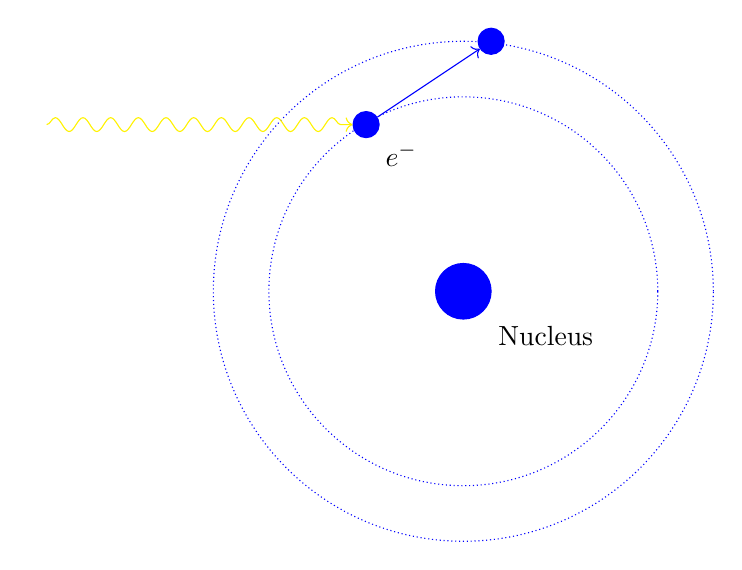
\begin{tikzpicture}
  \filldraw[fill=blue, draw=blue, outer sep = 3px] (0,0) circle (10px) node[label=below right:Nucleus]{};%{\small Nucleus};
  \path[densely dotted, draw=blue] (0,0) circle (70px);
    \path[densely dotted, draw=blue] (0,0) circle (90px);
  % \filldraw[fill=blue, draw=blue] (-79px, 70px) circle (3px) node[anchor=north west]{\tiny \(e^-\)};
  \node[circle,minimum size=5px, radius=5px,fill=blue, draw=blue, label=below right:\(e^-\)] (e1) at (-35px, 60px) {} ;
  \draw[->,decorate, decoration=snake, draw=yellow] (-150px, 60px) node[anchor=south east]{} -- (e1);
  \node[circle, radius=5px,fill=blue, draw=blue, label=below:\phantom{\(e^-\)}] (e2) at (10px, 90px) {} ;
  \draw[->, draw=blue] (e1) -- (e2);
\end{tikzpicture}
\end{document}